\documentclass{article}
\usepackage[utf8]{inputenc}
\usepackage{fullpage}
\usepackage{graphicx}
\usepackage{hyperref}
\usepackage{wrapfig}
\usepackage{fancyhdr}
\usepackage[ 
left=2.5cm,
right=2.5cm, 
top=3cm, 
bottom=3cm,
headheight = 3.5\baselineskip,
headsep = 5mm,
a4paper
]{geometry}

\setlength{\headheight}{16pt}
\pagestyle{fancy}
\renewcommand{\headrulewidth}{0.2pt} % no line in header area
\fancyhead{}
\pagestyle{fancy}
\fancyhf{}
\lhead{Computational Aspects of Digital Fabrication}
\rhead{Jan Pokorný}
\rfoot{\thepage}
\title{Dosimeter game}
\begin{document}

{\huge{Dosimeter game: Info sheet}}

\begin{center}
    \centering
    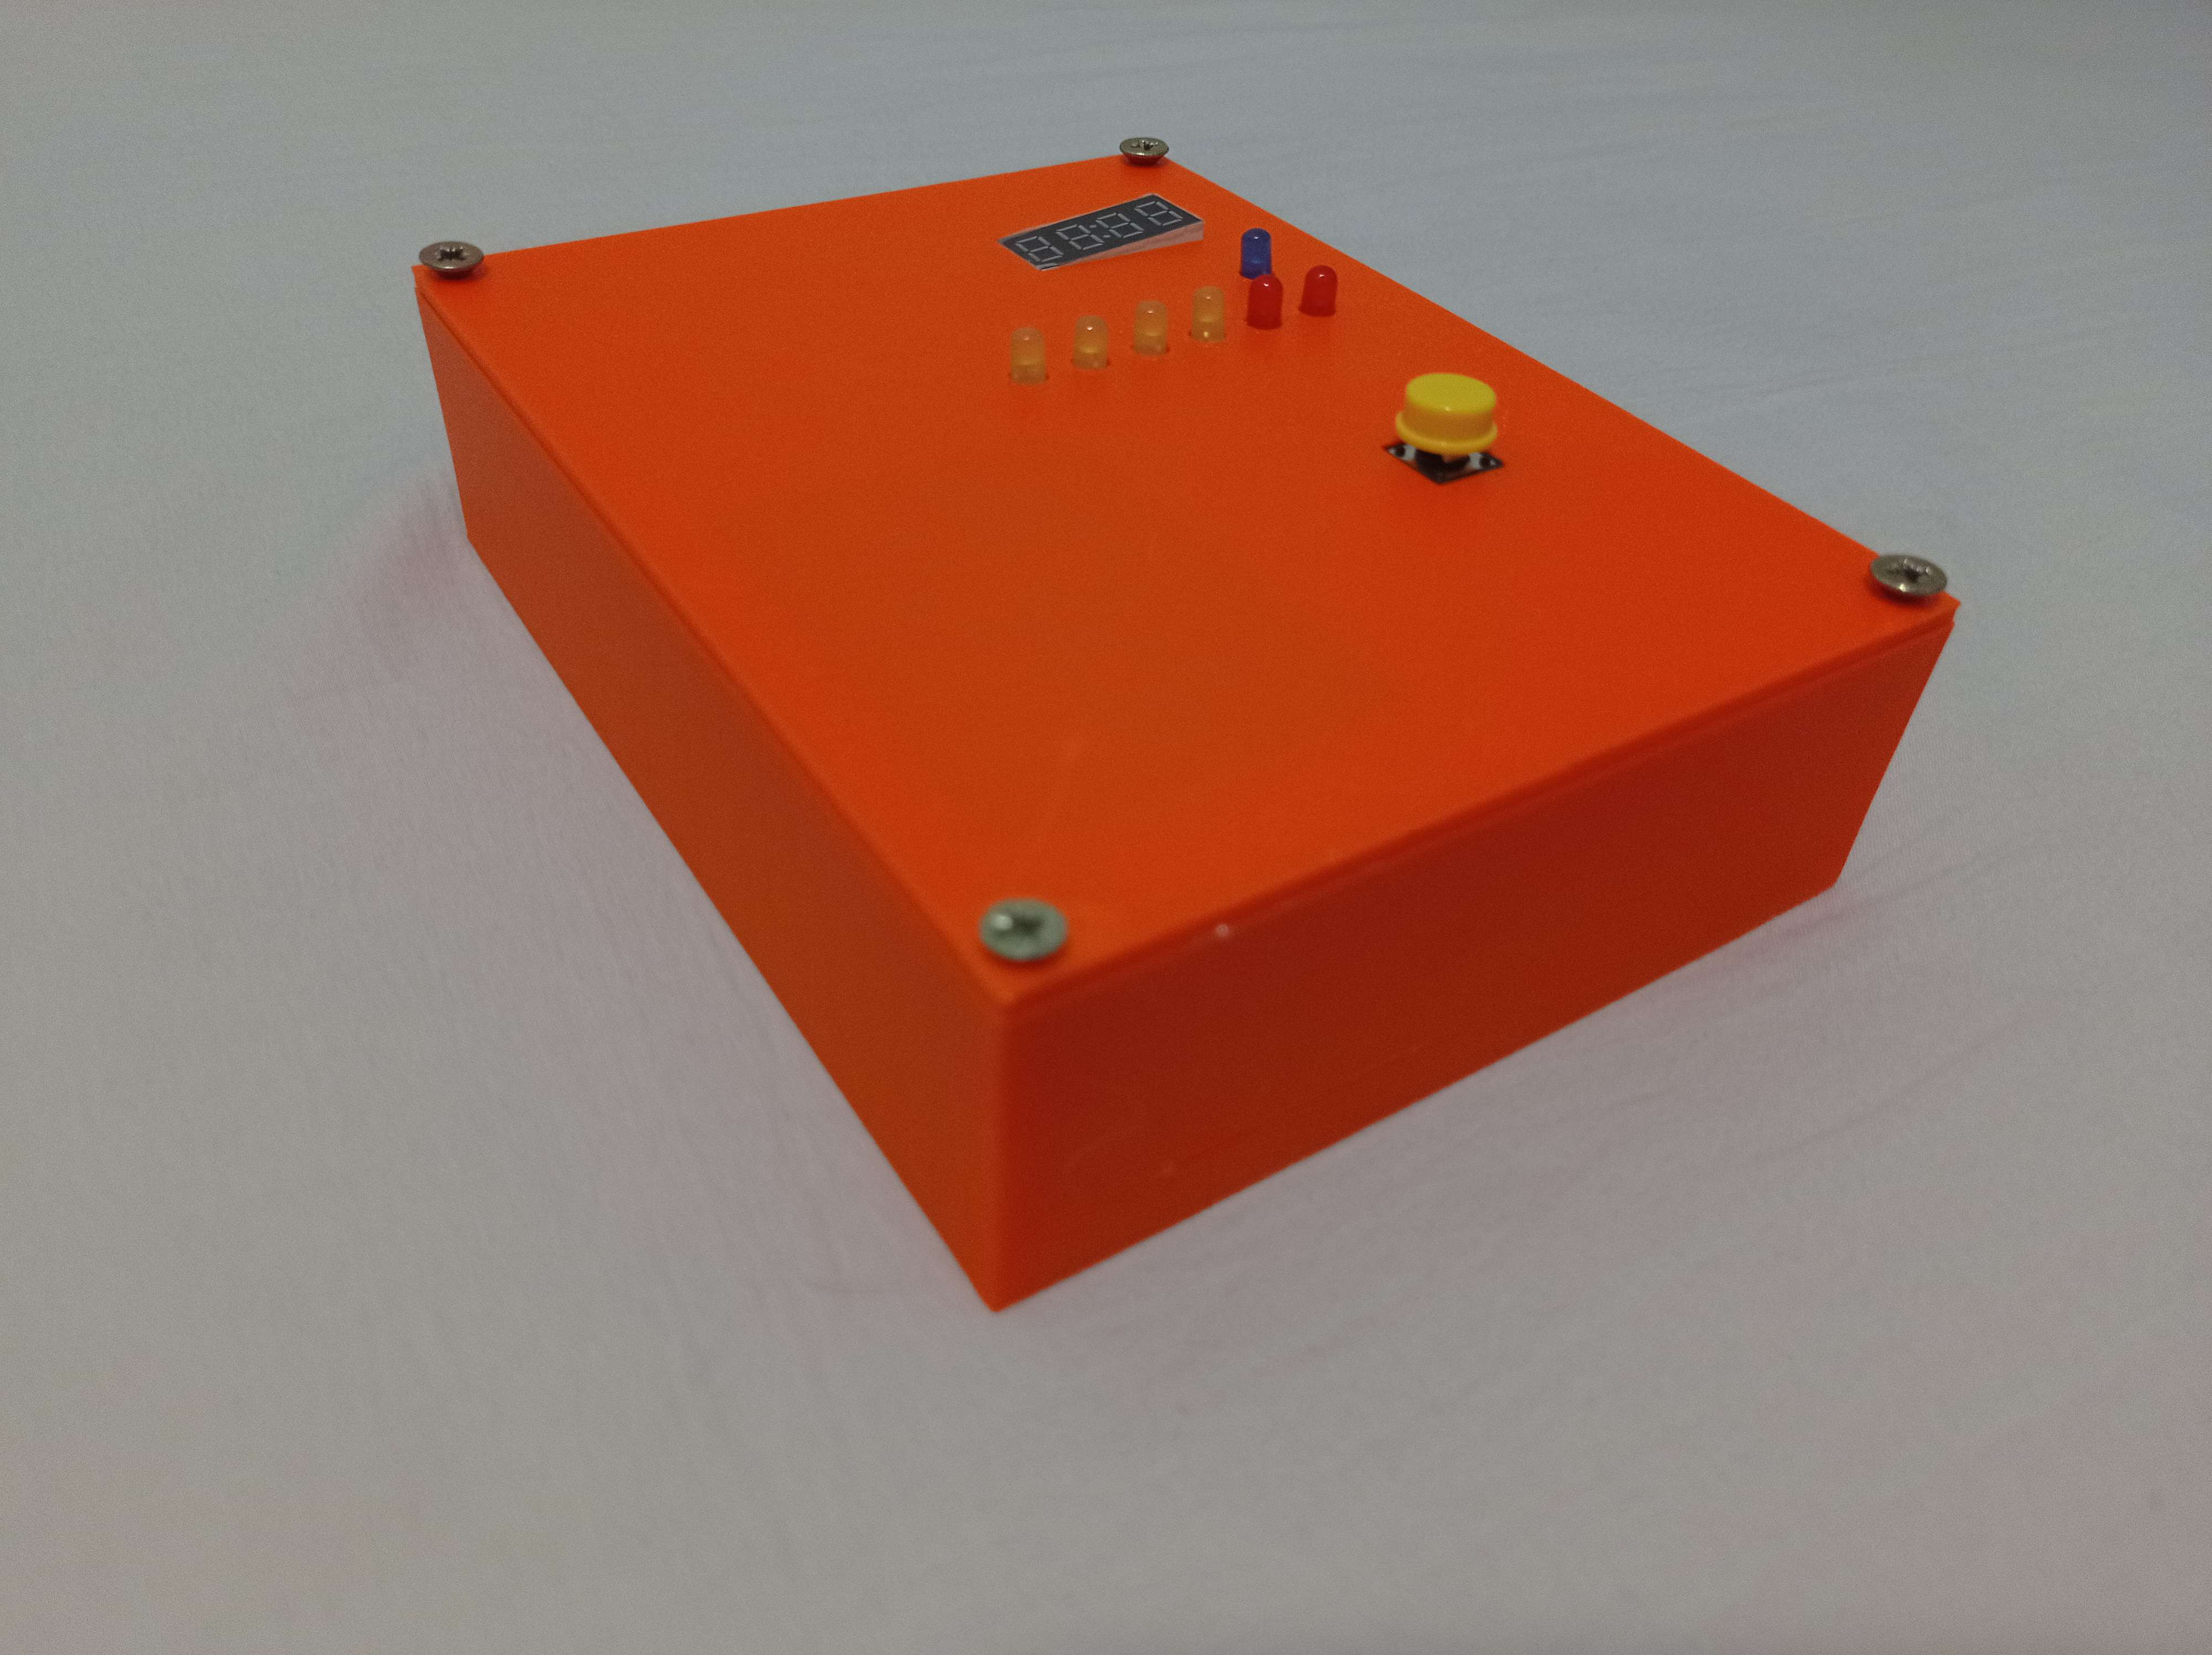
\includegraphics[width=0.5\textwidth]{imgs/Box2.jpg}
\end{center}

\section{Game}
The goal of the game is to survive and find a NFC tag. 
The player gathers information about its surrounding through a device.
The device gives the player a rough distance from the goal item and a strength of the radiation.
If the player is area with radiation, he loses health points.
If the health points of the player ever reaches a zero, the game is over.

\subsection{Controls}
\begin{enumerate}
\item Use the NFC card to restart the device by putting it next to the NFC reader (slightly darker rectangle, left of the button).
\item Press the button to change the displayed information. THe display displays these types of information:
\begin{itemize}
\item Goal(G): The distance (not in meters - signal strength from the ) from the goal.
\item Time: Time since the beggining of the game.
\item Radiation(r): Amount of radiation the player is receiving. The higher the radiation, the faster loses the player health points. 
\item Health(H): Number of health points remaining, if this counter reaches zero, the game ends.
The letter in parenthesis is displayed as the first character on the display.
\end{itemize}
\item Monitor the health bar, the less LEDs are lit up, the lower the amount of health points the player has.
\item Find the NFC tag and put it next to the NFC reader. The display now shows how fast you were.
\end{enumerate}

\emph{Be carefully with the device, too quick movements with it may damage the components inside.}

\section{How to make}
    The creation process includes 3D modeling and printing of the custom box of the device as well as programing of a microprocessor as the tool of digital fabrication.
    Other employed techniques are soldering and hot gun gluing.

\begin{wrapfigure}{r}{0.5\textwidth}
    \centering
    \includegraphics[width=0.4\textwidth]{imgs/Sketch.png}
    \caption{First sketch of the device.}
\end{wrapfigure}

\subsection{Components}
The main components are:
\begin{itemize}
    \item RaspberryPi 4 B
    \item 4 Digit Display V1.2 (HW-069) 
    \item RFID-RC522
    \item Powerbank
\end{itemize}
Furthemore, standard components for RPi as LEDs, button, cables were used.

\subsection{PIN layout} \label{pins}
\begin{itemize}
    \item Digit Display V1.2 (HW-069)
        \begin{itemize}
            \item CLK - GPIO 3 (5)
            \item DIO - GPIO 2 (3)
            \item VCC - 3.3V (1)
            \item GND - GND(6)
        \end{itemize}
    \item RFID-RC522
        \begin{itemize}
            \item SDA - GPIO 8 (24)
            \item SCK - GPIO 11 (23)
            \item MOSI - GPIO 10 (19)
            \item MISO - GPIO 9 (21)
            \item IRQ - Not used
            \item GND - GND (20)
            \item RST - GPIO 25 (22)
            \item 3.3V - 3.3V (17)
        \end{itemize}
    \item Button
        \begin{itemize}
            \item Power - 5V (4)
            \item Detect - GPIO 4 (7)
        \end{itemize}
    \item LEDS
        \begin{itemize}
            \item L1 - GPIO 5 (29)
            \item L2 - GPIO 6 (31)
            \item L3 - GPIO 13 (33)
            \item L4 - GPIO 19 (35)
            \item L5 - GPIO 26 (37)
            \item L6 - GPIO 20 (38)
            \item Status - GPIO 21 (40)
            \item GND - GND (39)
        \end{itemize}
\end{itemize}

\subsection{Extra components}
To be able to play the game you additionally need NFC tags and devices capable to emit Wi-fi signal.

The device is able to detect the Wi-fi networks automatically if you name them \texttt{DM-radiation} and \texttt{DM-goal} to be listed as the radiation and goal respectively. 
It is also possible to specify their ESSID in the \texttt{config.json}.
The NFC tags have to be named correctly:
\begin{itemize}
    \item \texttt{HP} -- sets the player health points to 100.
    \item \texttt{RESET} -- restarts the game.
    \item \texttt{GOAL} -- wins the game.
\end{itemize}
To name the tags, the file \texttt{write.json} may be used.

\subsection{Tutorial}
    Depending on the exact components used, the device may differ.
    The provided STL \texttt{models/box.stl} expects standard Arduino/RaspberryPi LEDs nad button and 43x91 mm powerbank.
    To adjust the 3D model, change parameters in \texttt{models/box.scad} using \emph{OpenSCAD}.
    Both models are contained in a single file to be able to see how components line up.
    For printing the model has to be split up into two pieces and rotated correspondingly. 

\begin{figure}[ht]
    \centering
    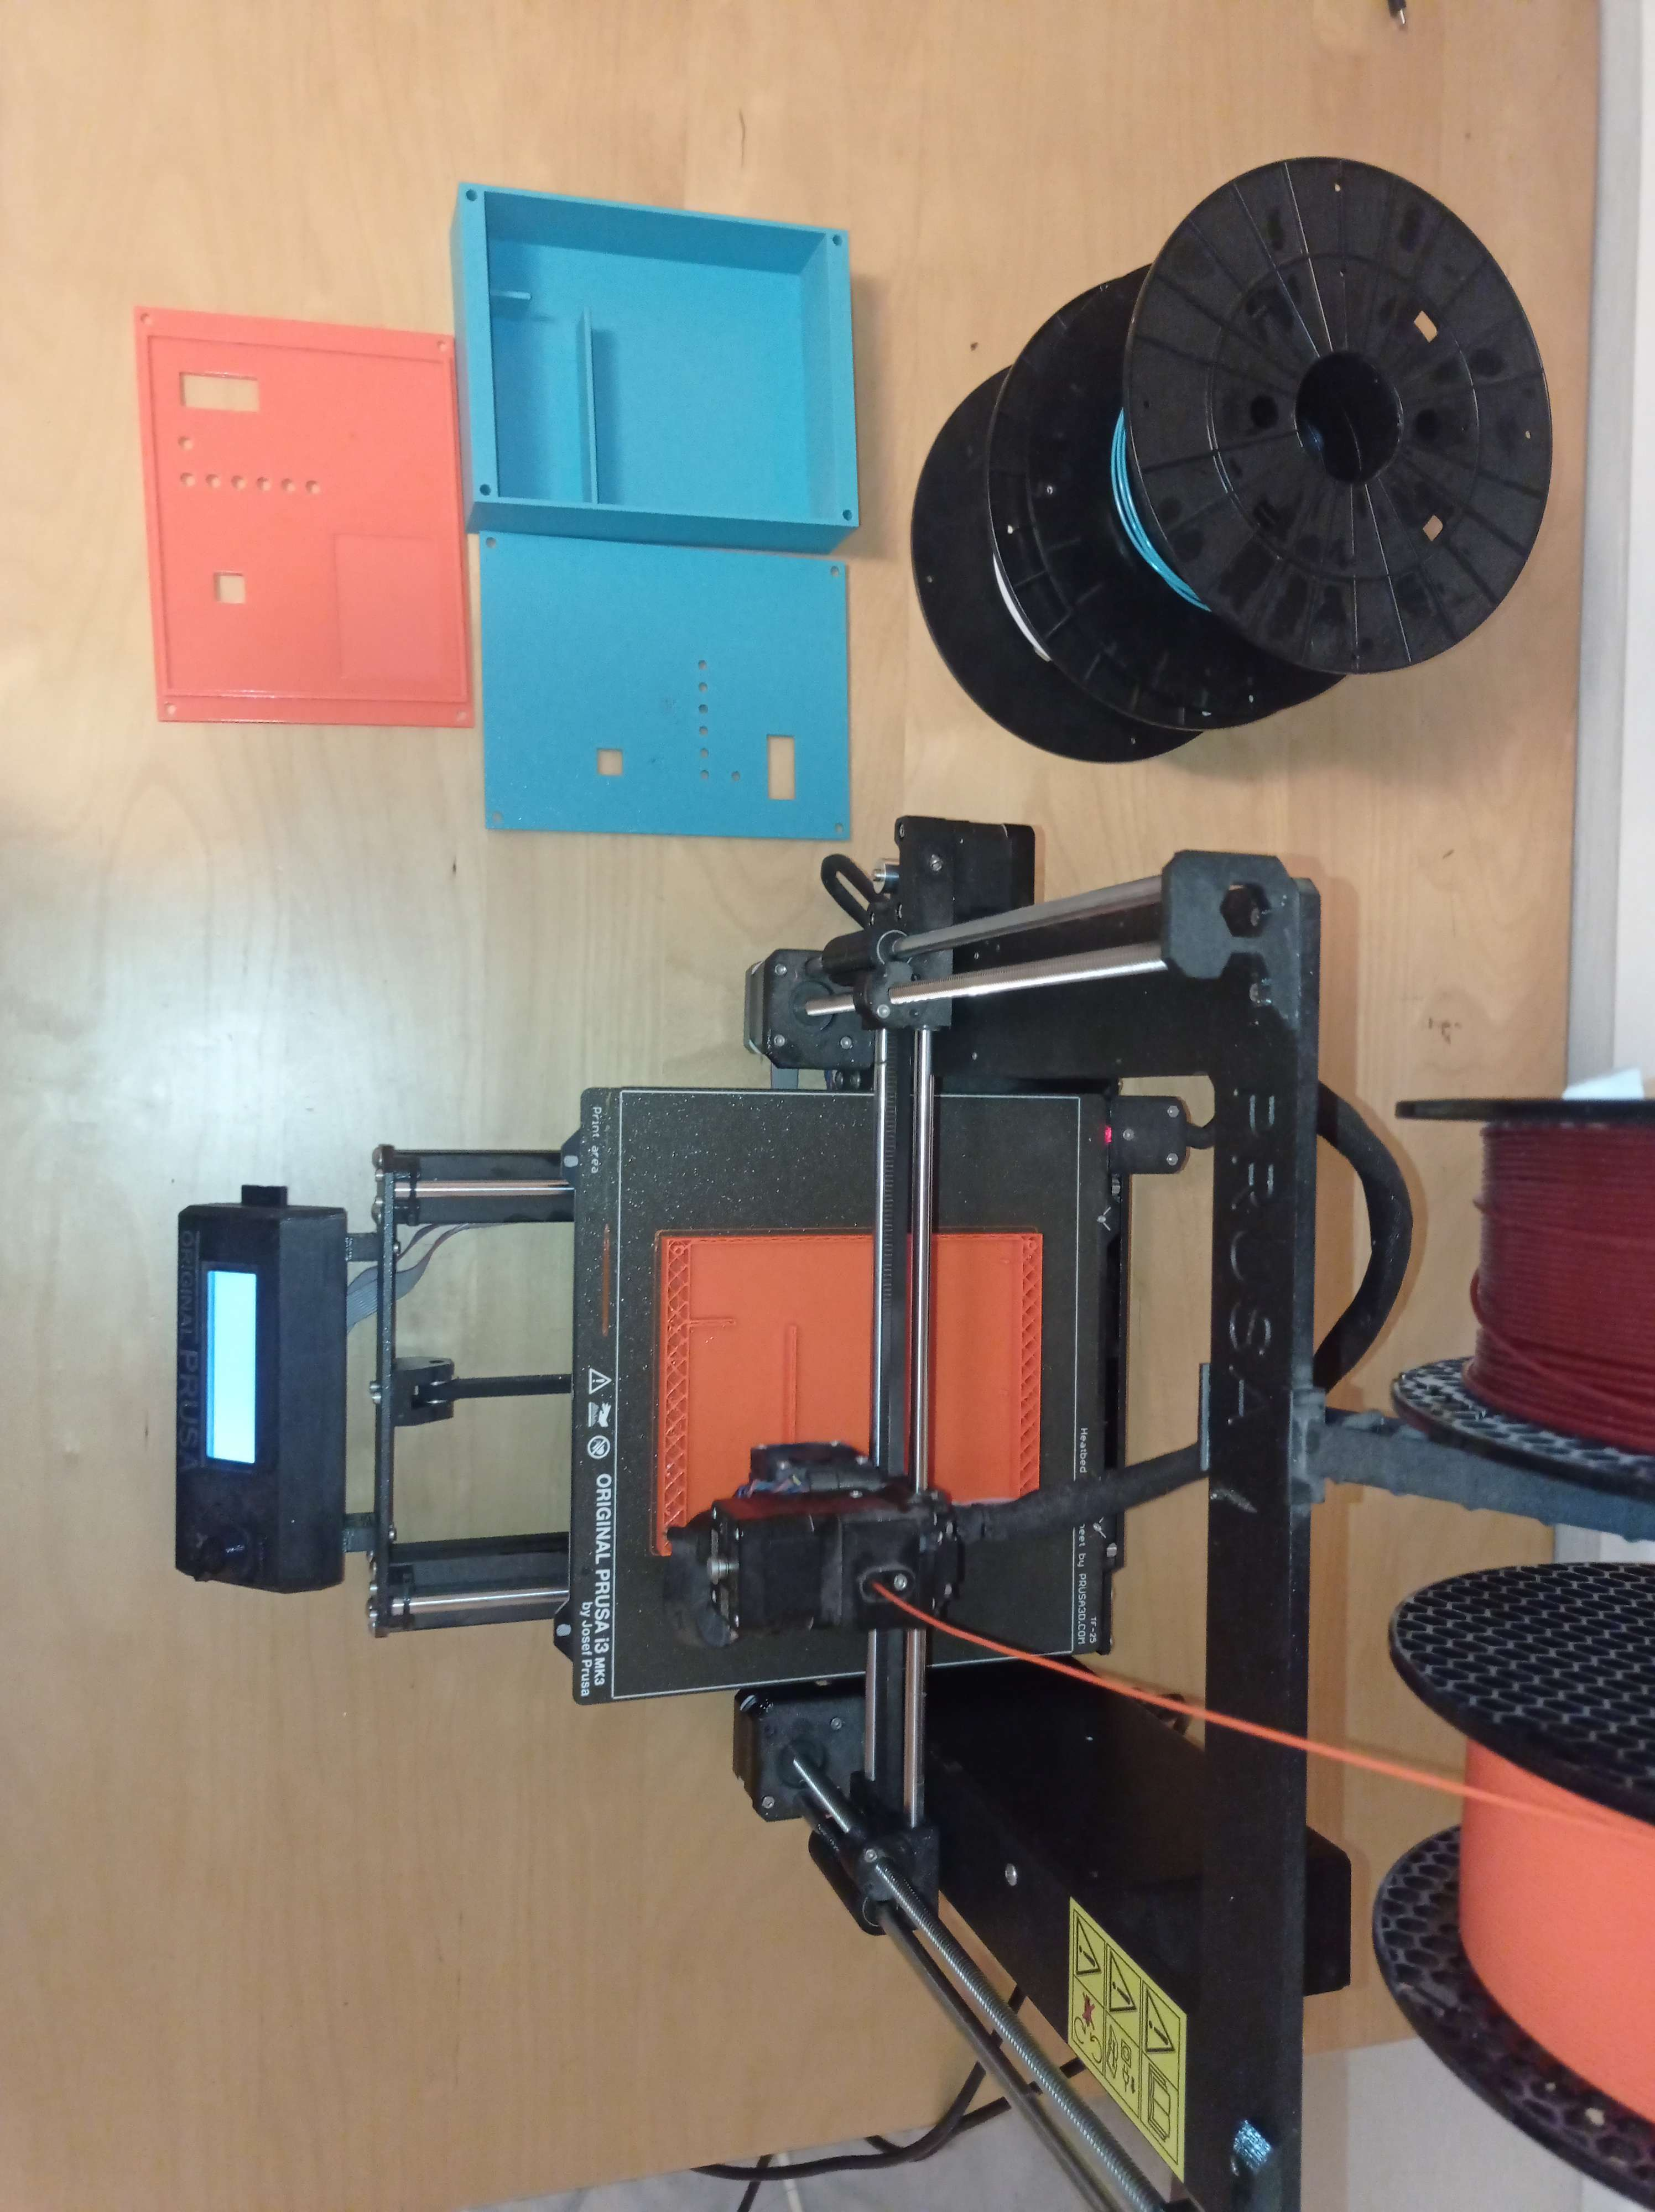
\includegraphics[width=0.5\textwidth]{imgs/Printing.jpg}
    \caption{3D printing of provided models.}
\end{figure}

    The component \emph{RFID-RC522} has to be soldered. 
\begin{figure}[ht]
    \centering
    \begin{tabular}{cc}
        \label{soldering}
        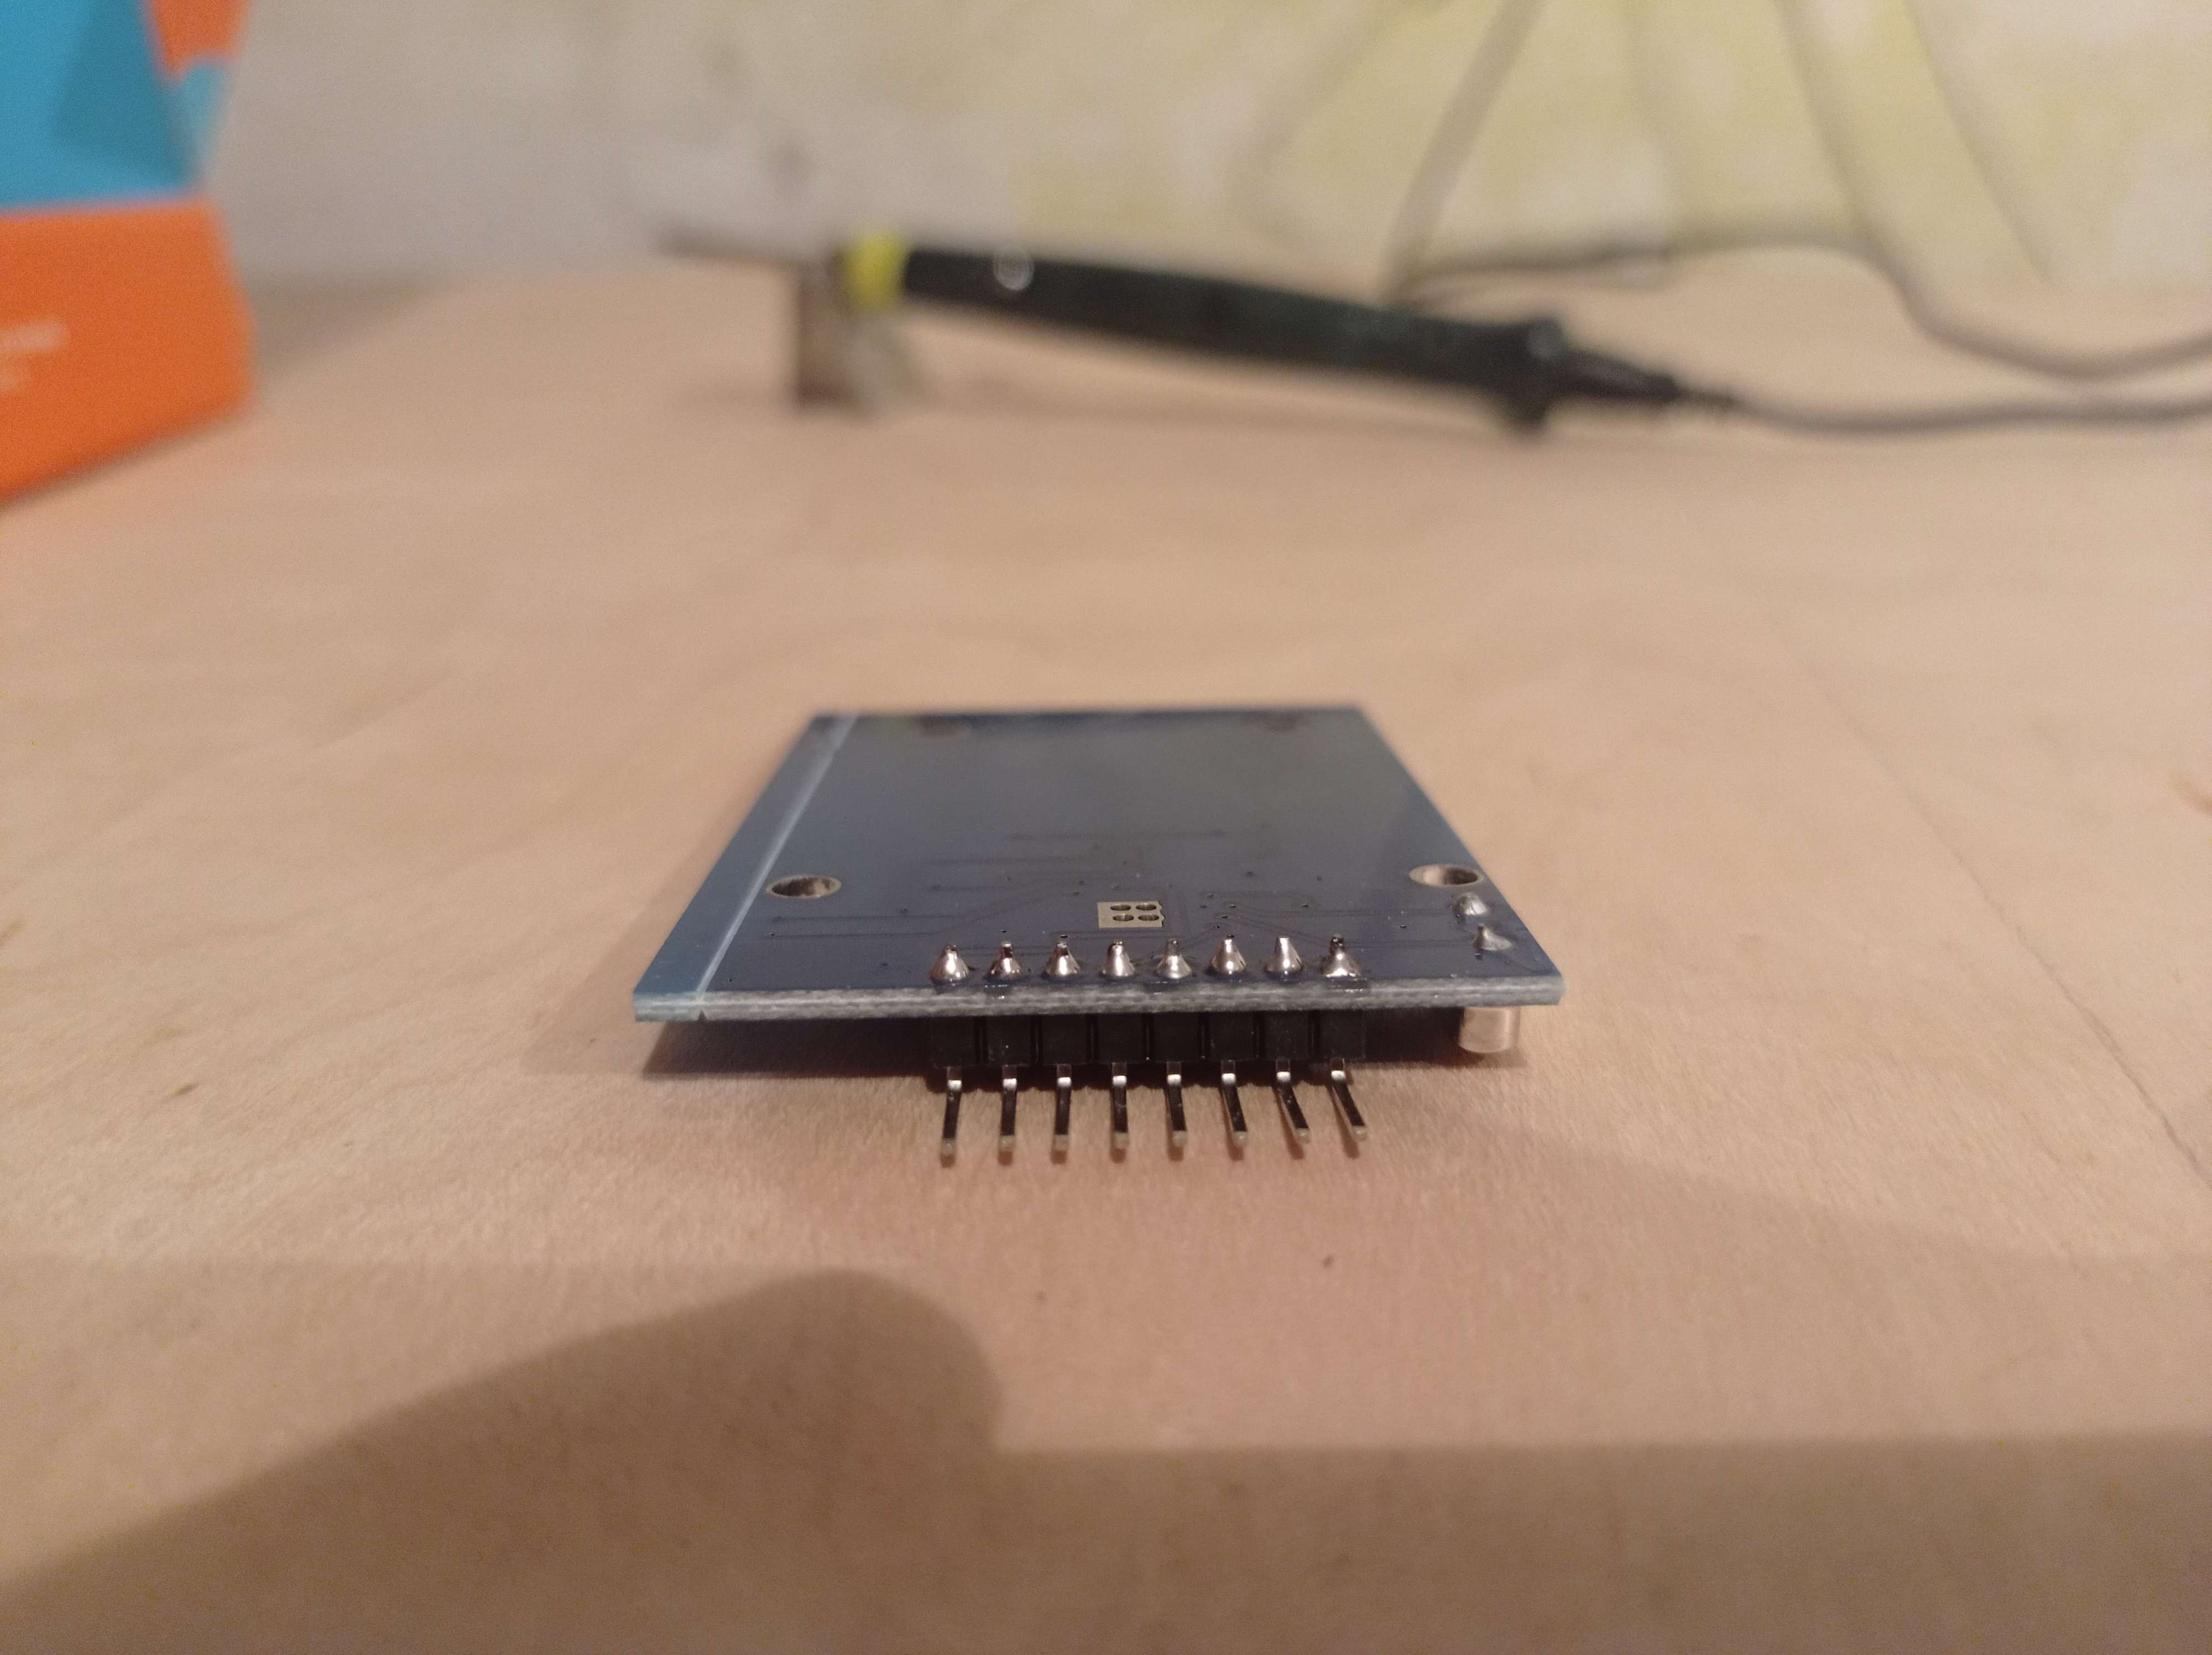
\includegraphics[width=0.53\textwidth]{imgs/Soldering1.jpg}
        &
        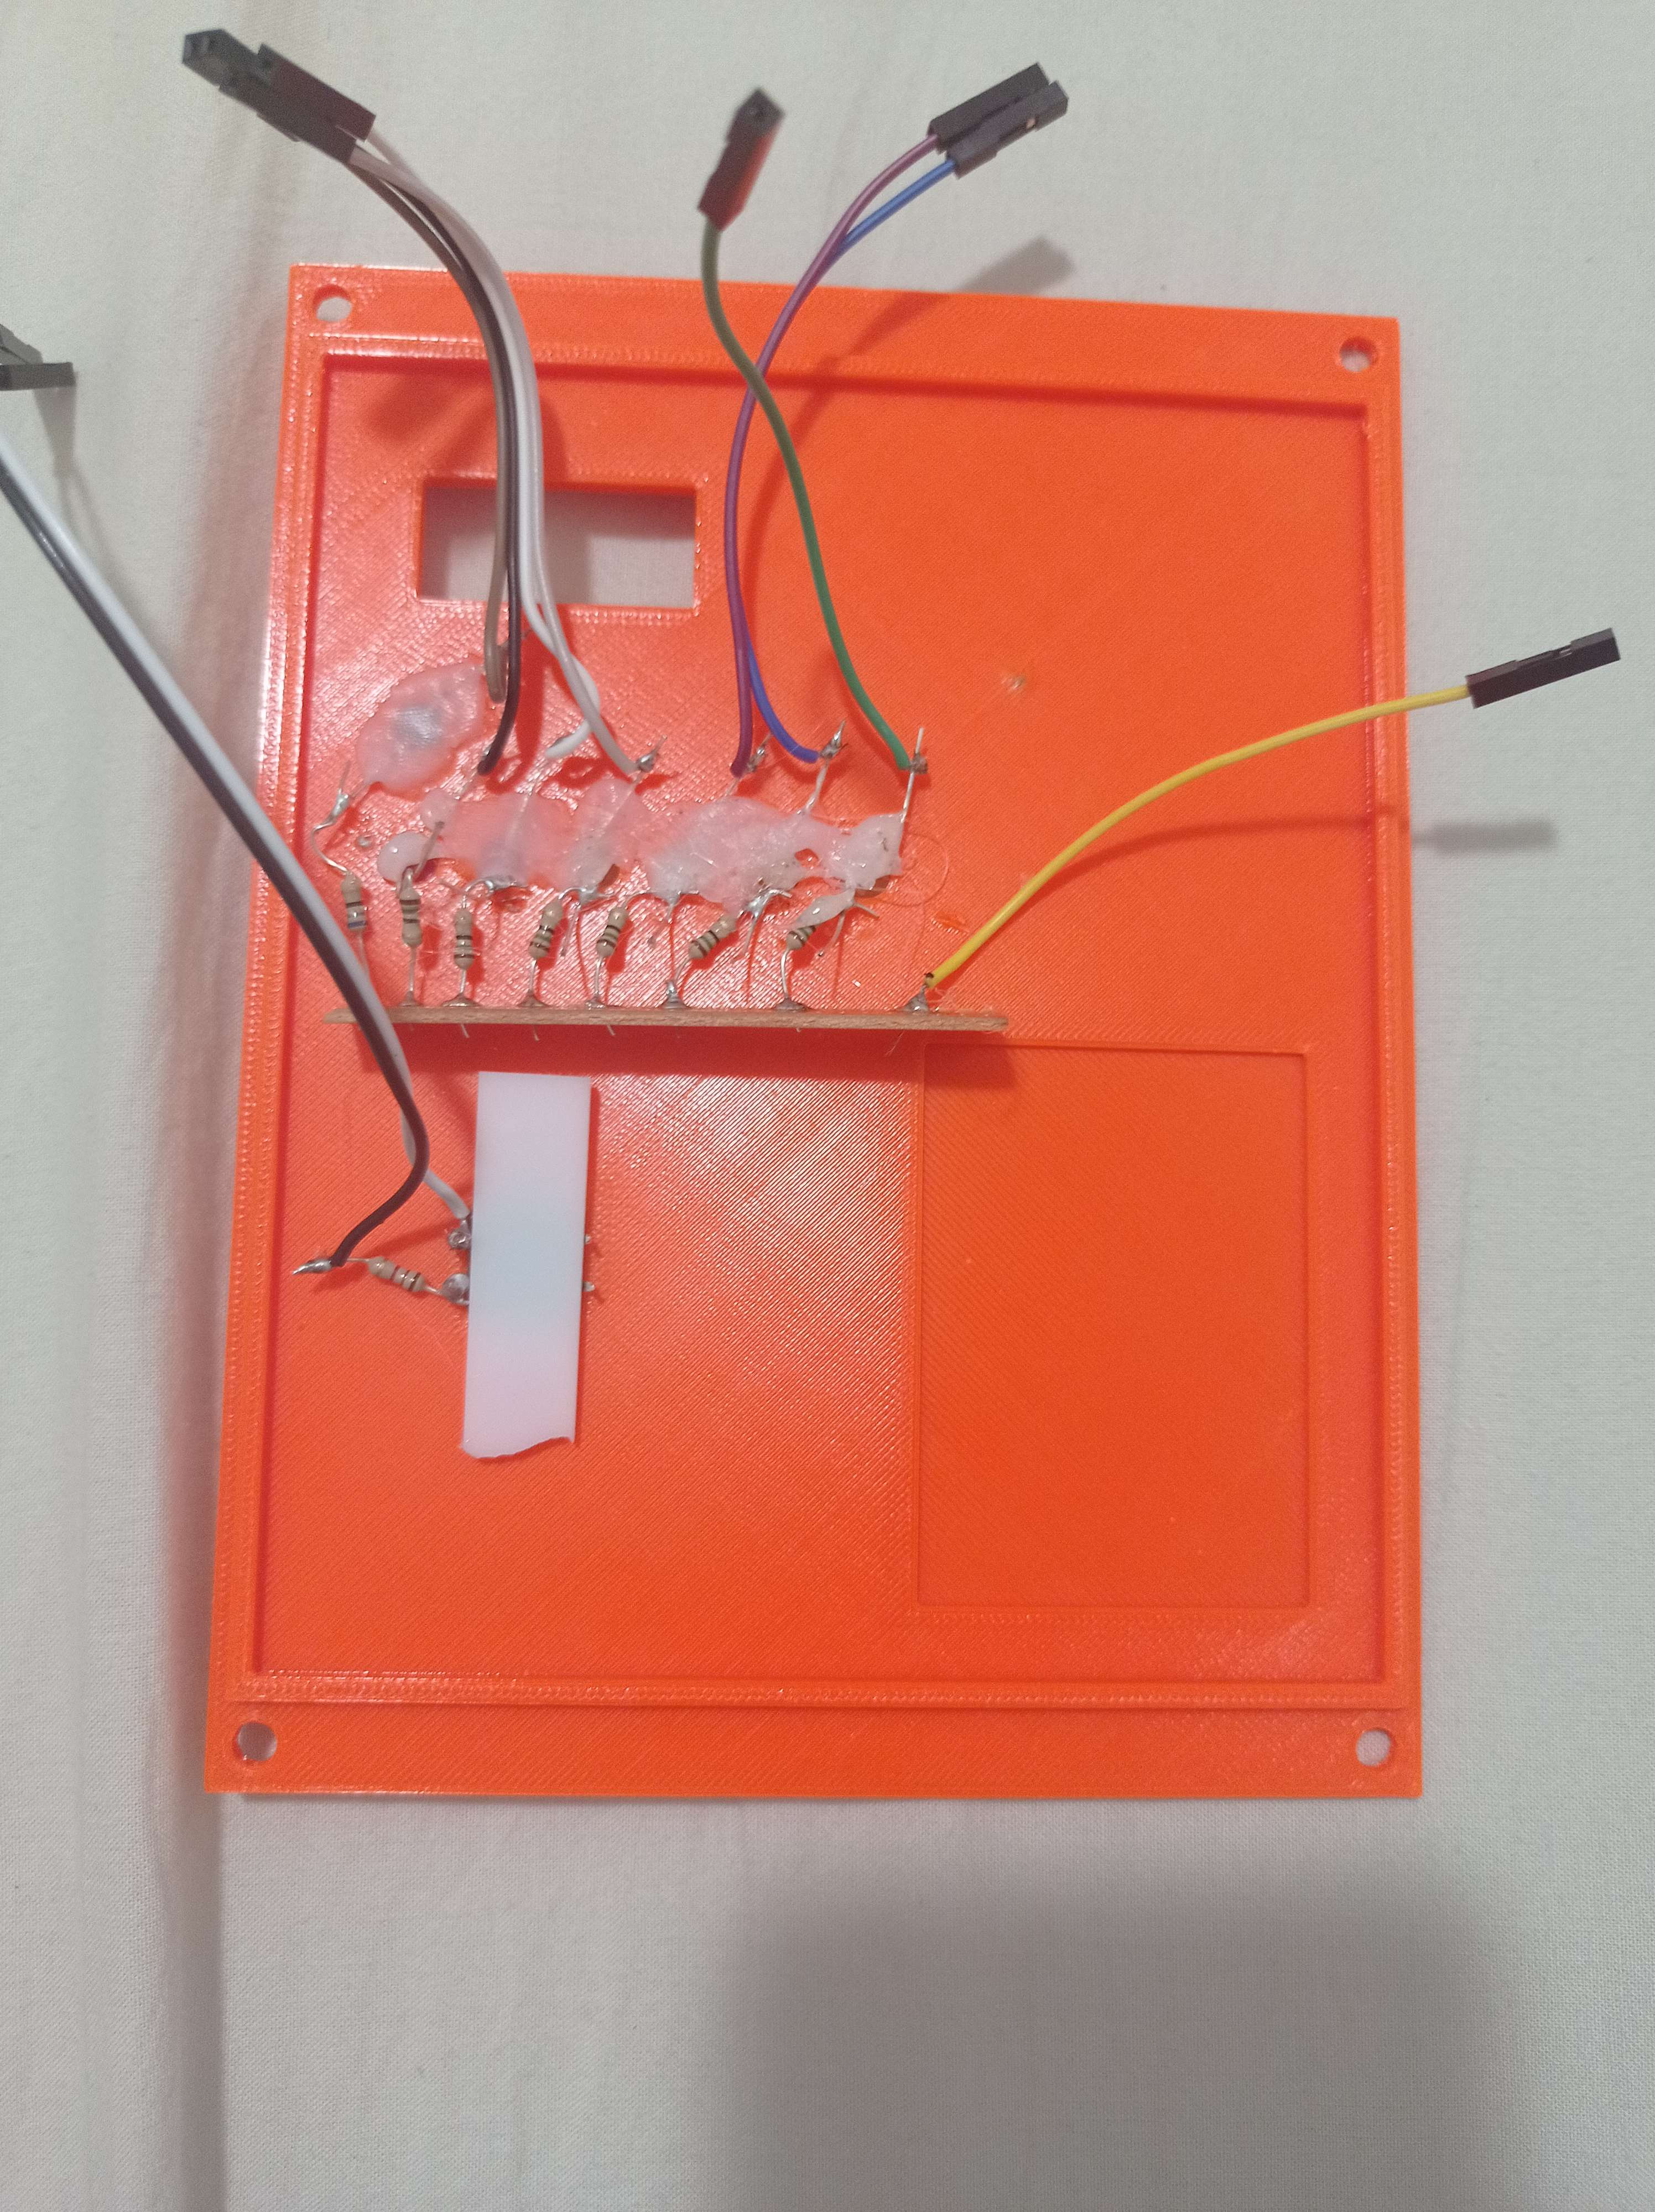
\includegraphics[width=0.3\textwidth]{imgs/Soldering2.jpg}
    \end{tabular}
    \caption{Soldering of the component \emph{RFID-RC522}on the left and soldering of the LEDS and the button on the right.}
\end{figure}

    Every LED is connected with a resistor to adjust the amount of current it goes through. 
    All LEDS are connected to a shared ground (yellow) and each of them has its own controlling pin.
    They are connected to the upper box part by a glue gun.
    The button is permanently attached with by a glue gun as well.
    The exact wiring is shown in figure \ref{soldering} and then in figure \ref{wiring}.

    Every component is connected to the RaspberryPi as described in section \ref{pins}. 
    The display is attached to the upper part of the box with tight fit.
    The NFC reader is attached by a clear sticky tape.

\begin{figure}[ht]
    \label{wiring}
    \centering
    \begin{tabular}{cc}
        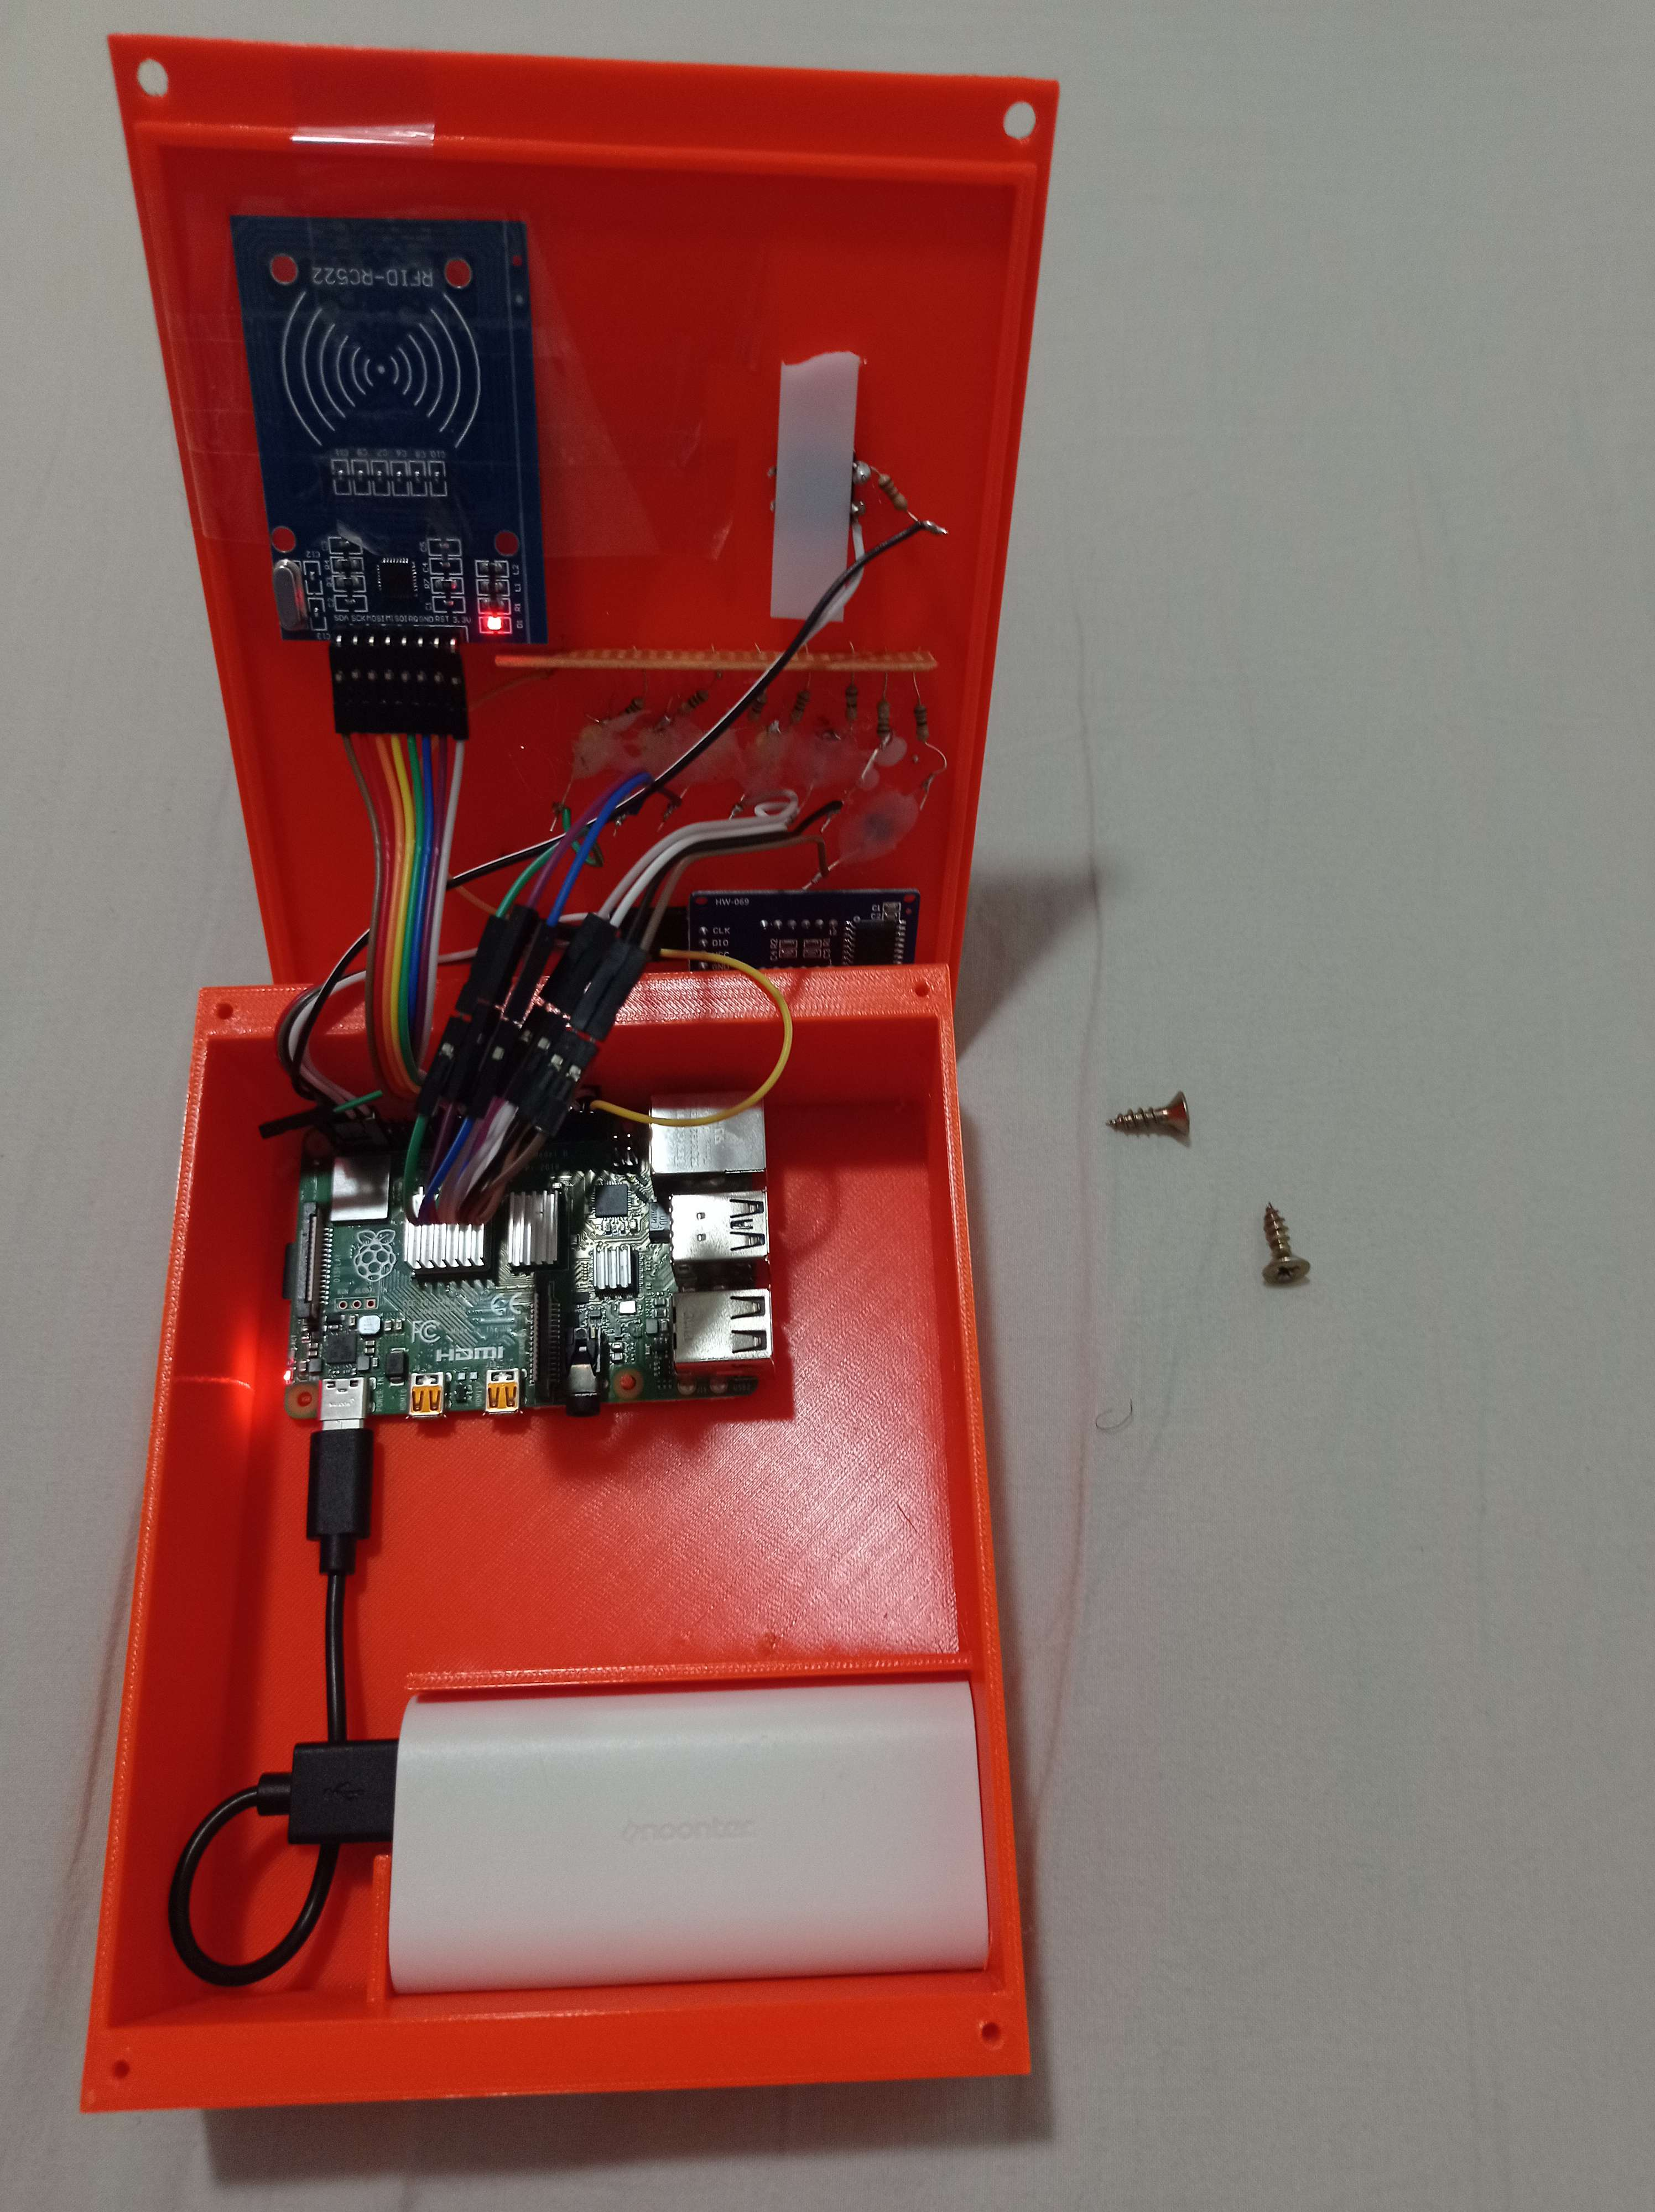
\includegraphics[width=0.5\textwidth]{imgs/Inside.jpg}
        &
        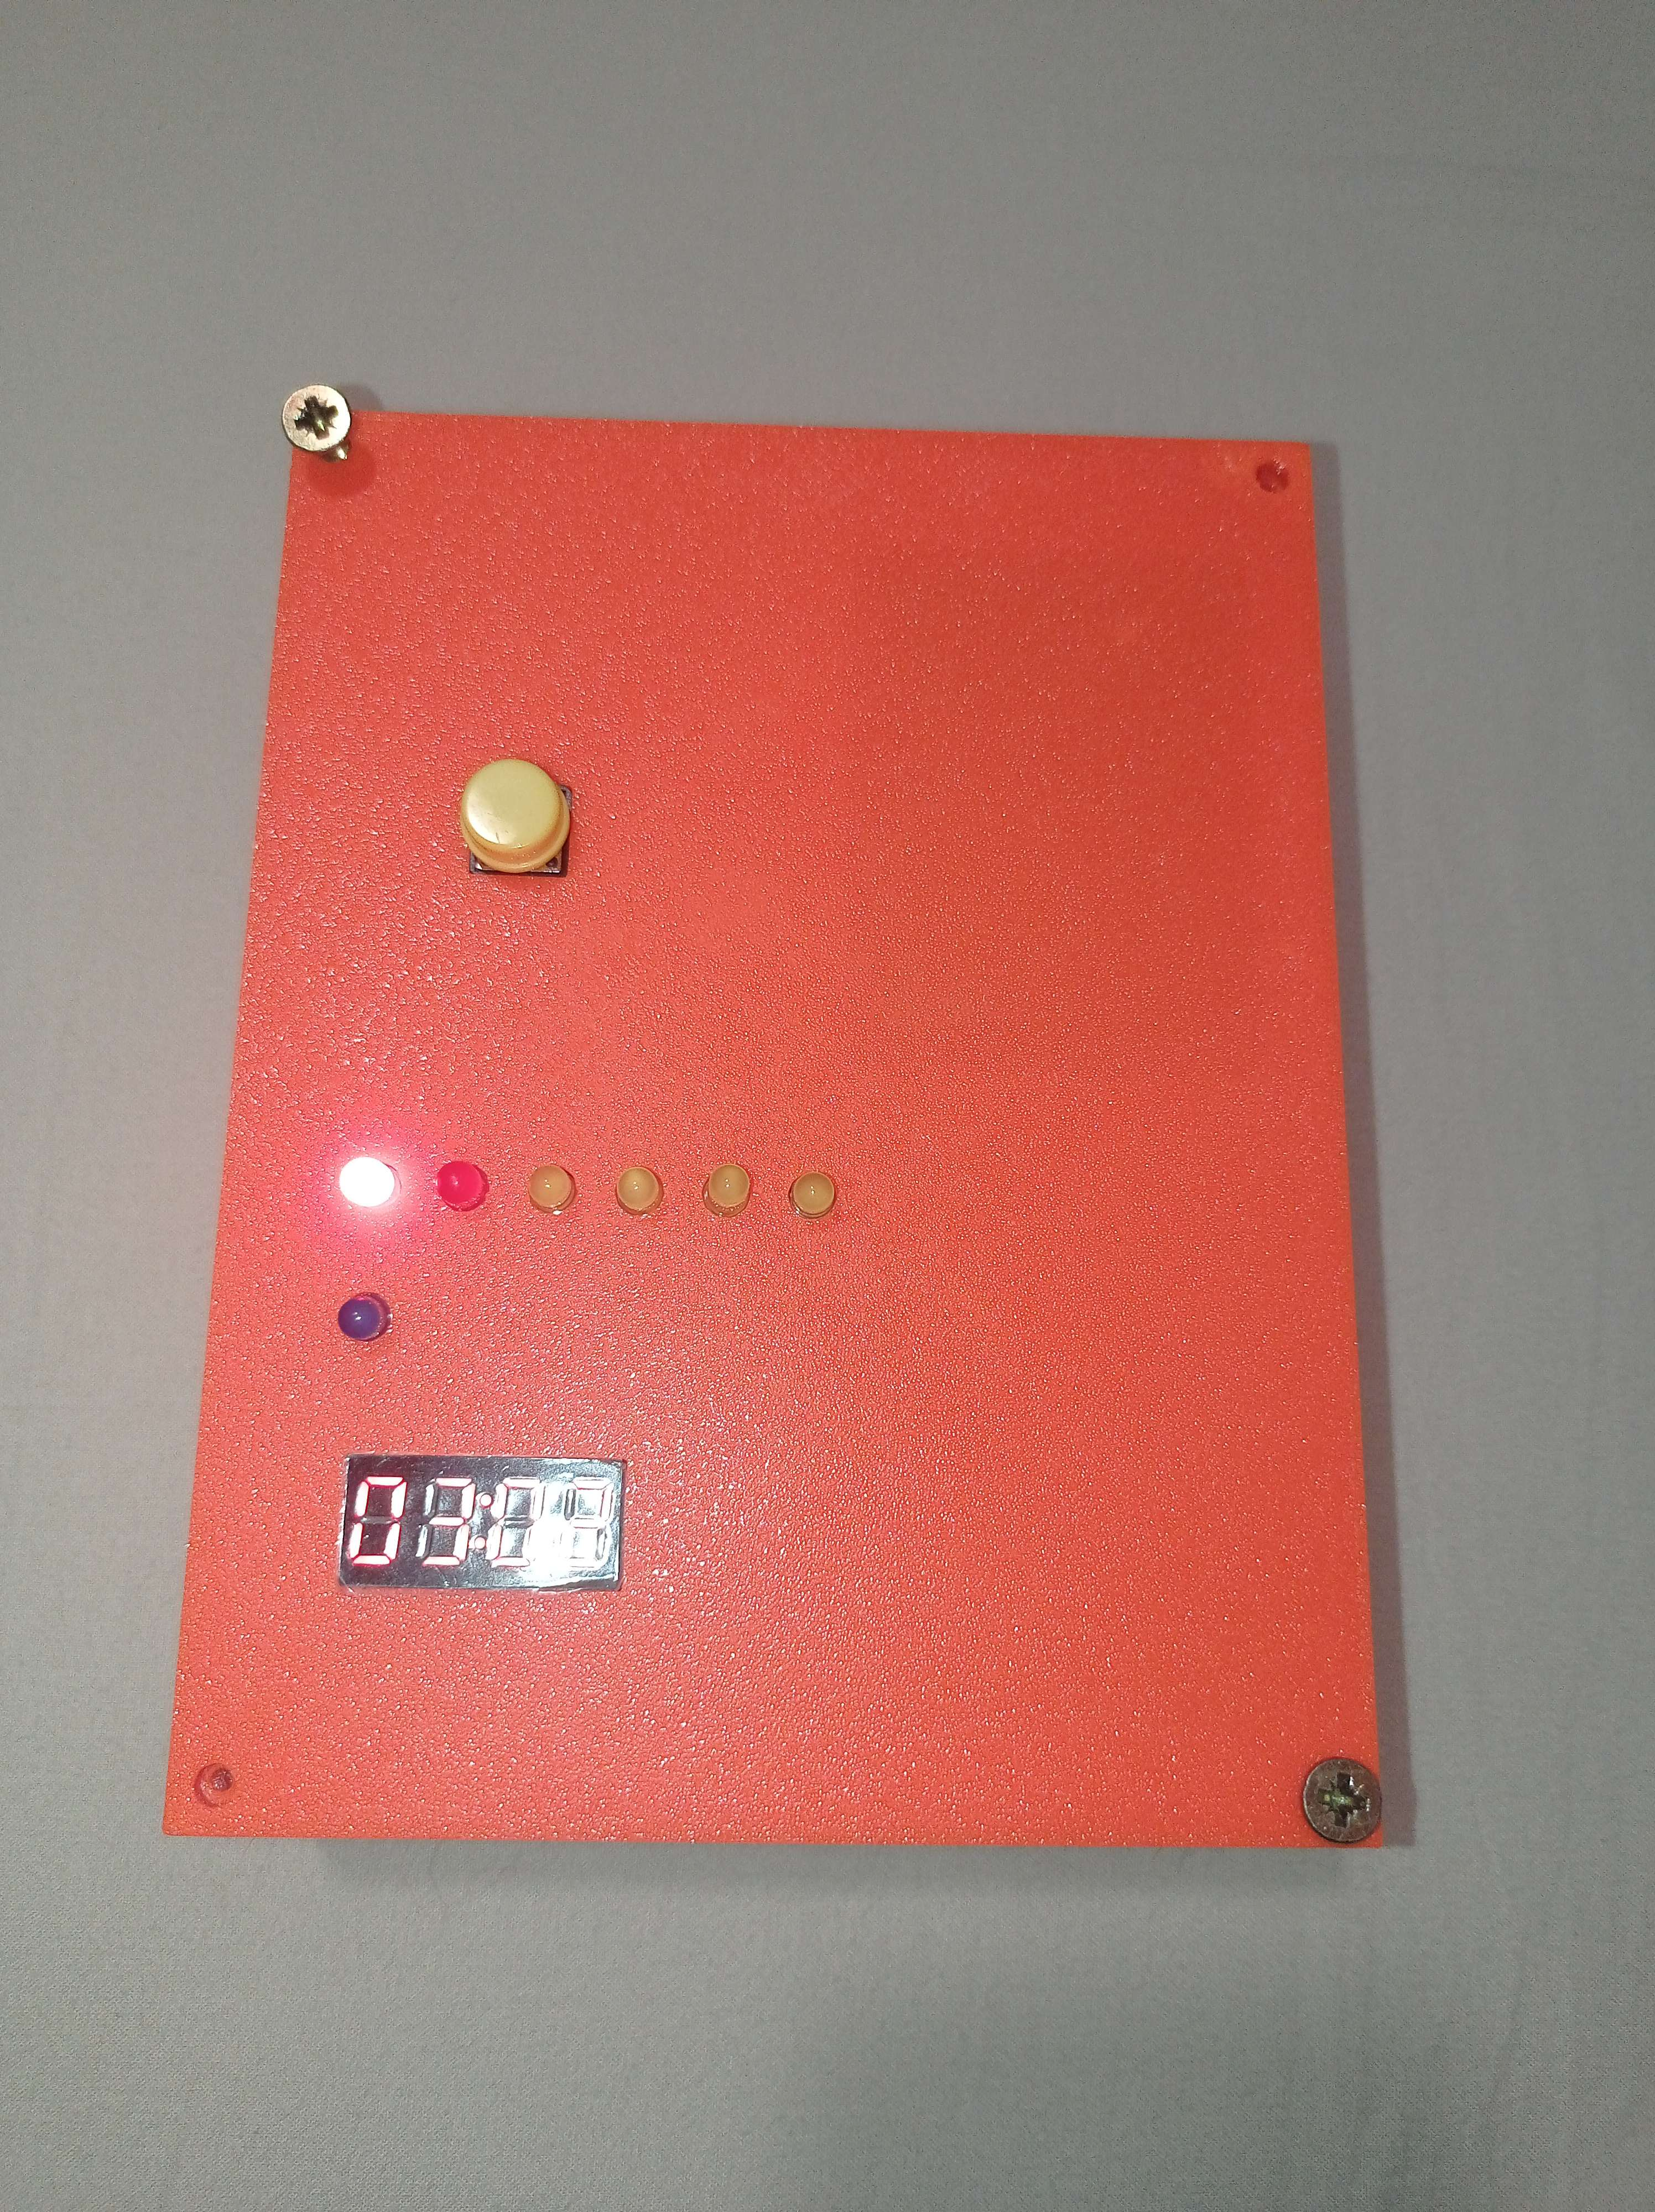
\includegraphics[width=0.5\textwidth]{imgs/Box1.jpg}
    \end{tabular}
    \caption{The device from the inside on the left and completed running device on the right.}
\end{figure}

    To turn the device on run \texttt{main.py}.
    Required packages are listed in \texttt{requirements.txt}


    The code, models and other assets are on GitHub: \url{https://github.com/alfapark/Dosimeter-mock}.


\subsection{Declaration}
    The project was done entirely by its single author Jan Pokorny. 
    The involvement of other people was only through discussion of technical details amd borrowing of their equipment which I am thankful for.
\end{document}
